\documentclass[tikz, border=1pt]{standalone}

\usepackage{xcolor}
\usetikzlibrary{arrows.meta}
\begin{document}
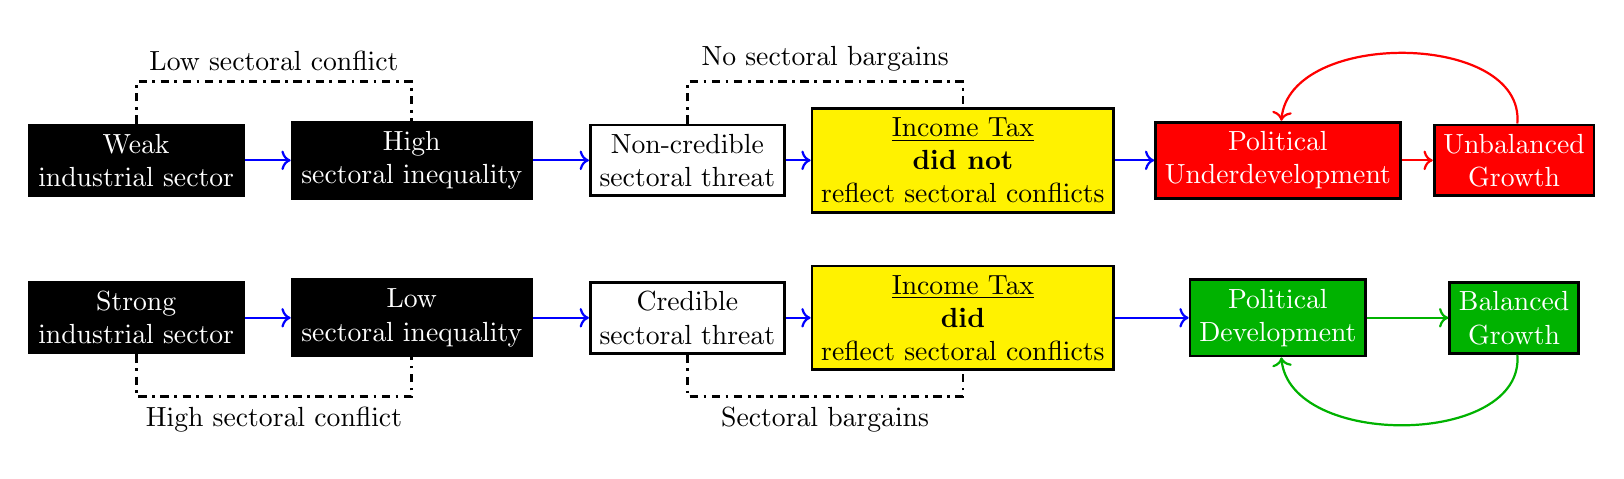
\begin{tikzpicture}[line width=1pt]


% 1
\node[draw,align=center,fill=black,text=white] (ArgumentA1) at (1,0) {Strong\\industrial sector};
\node[draw,align=center,fill=black,text=white] (ArgumentB1) at (4.5,0) {Low\\sectoral inequality};
\node[draw,align=center] (ArgumentC) at (8,0) {Credible\\sectoral threat};
\node[draw,align=center,fill=yellow,text=black] (ArgumentD1) at (11.5,0) {\underline{Income Tax}\\{\bf did}\\reflect sectoral conflicts};
%\node[draw,align=center] (ArgumentD3) at (8,-2) {Successful incorporation\\of both elites};
%\node[draw,fill=black!30!green,text=white] (ArgumentE1) at (20.5,0) {Strong state};

% 1
\node[draw,fill=black!30!green,text=white,align=center] (ArgumentA3) at (15.5,0) {Political\\Development};
\node[draw,fill=black!30!green,text=white,align=center] (ArgumentB3) at (18.5,0) {Balanced\\Growth};
\draw[<-,draw=black!30!green,thick] (ArgumentB3) to (ArgumentA3);
\draw[->,draw=black!30!green,thick] (ArgumentB3) to[out=-85,in=-85] (ArgumentA3);



\draw[->,draw=blue,thick] (ArgumentB1) to (ArgumentC);
\draw[<-,draw=blue,thick] (ArgumentD1) to (ArgumentC);
\draw[->,draw=blue,thick] (ArgumentD1) to (ArgumentA3);
%\draw[|-|,draw=blue,thick] (ArgumentC) to (ArgumentD3);
\draw[->,draw=blue,thick] (ArgumentA1) to (ArgumentB1);
%\draw[->,draw=blue,thick] (ArgumentB3) to (ArgumentE1);


\draw[dash dot] (ArgumentA1) -- ++(0,-1) -| (ArgumentB1) node[below, near start] {High sectoral conflict};

\draw[dash dot] (ArgumentC) -- ++(0,-1) -| (ArgumentD1) node[below, near start] {Sectoral bargains};
 

\node at (6., -1.0) {};










% 2
\node[draw,align=center,fill=black,text=white] (ArgumentA2) at (1,2) {Weak\\industrial sector};
\node[draw,align=center,fill=black,text=white] (ArgumentB2) at (4.5,2) {High\\sectoral inequality};
\node[draw,align=center] (ArgumentC) at (8,2) {Non-credible\\sectoral threat};
\node[draw,,align=center,fill=yellow,text=black] (ArgumentD2) at (11.5,2) {\underline{Income Tax}\\{\bf did not}\\reflect sectoral conflicts};


%\node[draw,align=center] (ArgumentD23) at (8,4) {Failure to incorporate\\both elites}; 

%\node[draw,fill=red,text=white] (ArgumentE2) at (20.5,2) {Failed state};

\node[draw,fill=red,text=white,align=center] (ArgumentA4) at (15.5,2) {Political\\Underdevelopment};
\node[draw,fill=red,text=white,align=center] (ArgumentB4) at (18.5,2) {Unbalanced\\Growth};
\draw[<-,draw=red,thick] (ArgumentB4) to (ArgumentA4);
\draw[->,draw=red,thick] (ArgumentB4) to[out=85,in=85] (ArgumentA4);


\draw[->,draw=blue,thick] (ArgumentD2) to (ArgumentA4);
%\draw[|-|,draw=blue,thick] (ArgumentC) to (ArgumentD23);

%\draw[->,draw=blue,thick] (ArgumentB4) to (ArgumentE2);




\draw[->,draw=blue,thick] (ArgumentB2) to (ArgumentC);
\draw[<-,draw=blue,thick] (ArgumentD2) to (ArgumentC);
\draw[->,draw=blue,thick] (ArgumentA2) to (ArgumentB2);

\draw[dash dot] (ArgumentA2) -- ++(0,1) -| (ArgumentB2)
node[above, near start] {Low sectoral conflict};

\draw[dash dot] (ArgumentC) -- ++(0,1) -| (ArgumentD2) node[above, near start] {No sectoral bargains}; % here

\node at (6., -1.0) {};












  
\end{tikzpicture}
\end{document}